\section{What Grid Computing is}
Grid Computing is a type of Distributed Computing where the resources of many computers, connected by a network, are used in combination to reach a certain common goal.

\begin{figure}[!ht]
    \centering
    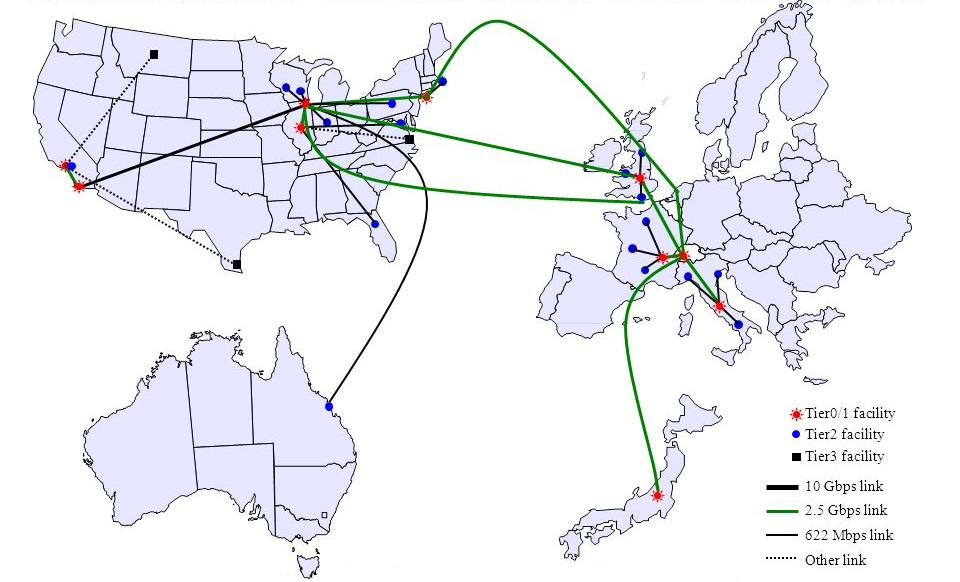
\includegraphics[scale=0.46]{document/chapters/chapter_1/images/iVDGL_globus.jpg}
    \caption{Example of a Grid - iVDGL, the Globus project \cite{iVDGL}}
    \label{fig:iVDGL}
\end{figure}

Compared to traditional Distributed Computing like Cluster Computing, Grid Computing focuses on large-scale resource with geographically dispersed nodes that also tend to be more heterogeneous regarding their hardware and software.
Another important aspect that differentiates Grid Computing from Cluster Computing is how the last one tends to be more focused on a particular task while the Grid is designed to a general-purpose tool.

\vspace{10mm}
\begin{figure}[!ht]
    \centering
    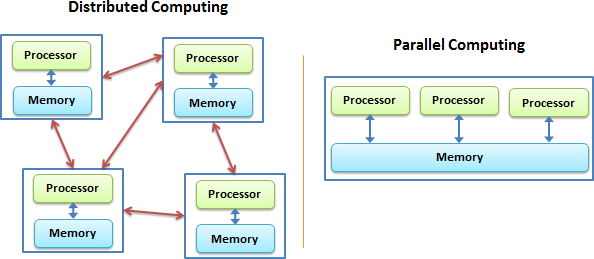
\includegraphics[width=\linewidth]{document/chapters/chapter_1/images/distributed_computing_vs_parallel_computing.png}
    \caption{High-level comparison of Distributed Computing and Parallel Computing \cite{distributed_vs_parallel}}
    \label{fig:distributed_vs_parallel}
\end{figure}
\vspace{7mm}

For certain applications, Grid Computing can be seen as a special type of Parallel Computing that distributes computation among the nodes connected to the Grid utilizing their resources; this approach is in contrast with the traditional notion of a supercomputer, which has many processors connected by a local high-speed bus.
From this difference in approach comes the strength of performing parallel computations in a distributed Grid environment: resources from the machines connected to the Grid can be quickly gathered to perform a task and, after completion, they can be dismantled just as quickly, removing the necessity of maintaining a highly expensive supercomputer; while this is, in a certain way, also true for Cluster Computing, the strength of Grid Computing lies in its ability to reach much greater levels of scalability with relative ease. 

\subsection{The "Grid problem"}
TODO

\subsection{History and applications using the Grid}
TODO